\chapter{Concurrency in C++}

\section{Threads}

\begin{paracol}{2}
   \begin{figure}[htbp]
      \centering
      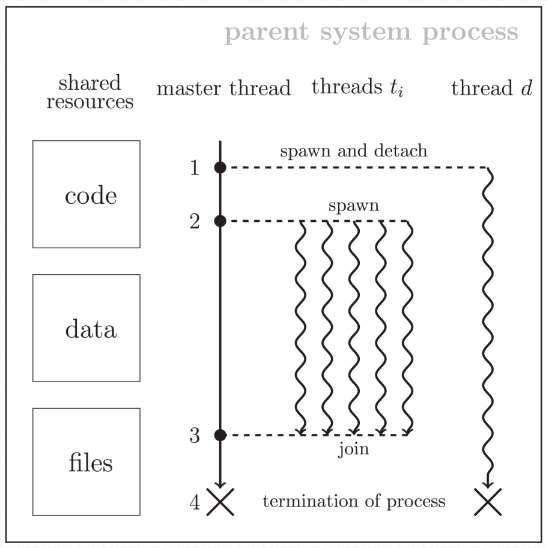
\includegraphics{images/08/threads1.png}
      \caption{Thread schema}
      \label{fig:08/threads1}
   
   \end{figure}
   
   \switchcolumn
   
   \begin{itemize}
      \item The master thread can spawn threads, and each thread can
   spawn threads as well
      \item The number of spawned threads should be roughly the
   amount of cores (i.e., pay attention to oversubscription)
      \item Threads share process resources
      \item each thread has a separate stack
      \item A thread can be joined or detached once
      \item A detached thread cannot be joined
      \item Joined or detached threads cannot be reused
      \item All threads must be joined or detached within the scope of
   their declaration
   \end{itemize}
\end{paracol}


% \begin{lstlisting}[caption={Hello World with threads}, label={lst:08/hello_world}]
% #include <cstdint>
% #include <thread>
% #include <vector>

% // uint64_t
% #include <iostream>  // std :: cout std :: endl
% // std :: vector
% // std: :thread

% // this function will be called by the threads (should be void)
% void say_hello(uint64_t id) {
%   std ::cout << "Hello from thread" << id << std ::endl;
% }
% // this runs in the master thread
% int main(int argc, char* argv[]) {
%   const uint64_t num_threads{(argc == 2) ? std ::stoul(argv[1]) : 10};
%   std ::vector<std ::thread> threads;

%   // for all threads
%   for (uint64_t id = 0; id < num threads; id++)
%     // emplace the thread object in vector threads
%     // using argument forwarding, this avoids unnecessary
%     // move operations to the vector after thread creation
%     threads.emplace_back(
%         // call say hello with argument id
%         say hello, id);

%   // join each thread at the end
%   for (auto& thread : threads) thread.join();
% }
%    \end{lstlisting}

%    \begin{itemize}
%       \item We need to store the thread handles explicitly to be able
%       to access them during the join phase
%       \item In the code snippet, we use a \lstinline|std::vector| container and
%       the method \lstinline|emplace_back|
%       \item Alternatively, we could have moved the thread object
%       implicitly using the vector member function \lstinline|push_back|
%       \item \lstinline|threads.push_back(std :: thread(say_hello, id));|
%       \item The type std::thread is move-only (i.e., not copyable)
%       \item How to compile:
%       \item \lstinline|g++ -O2 -std=c++17 hello_world.cpp -o hello_world -pthread|
%    \end{itemize}
   
\section{Asynchronicity and Tasks}
It may be more convenient to let the threads start asynchronously. This can be achieved by using the \lstinline|std::async| function. This function returns a \lstinline|std::future| object that can be used to retrieve the result of the function. The function is executed asynchronously, and the result is stored in the \lstinline|std::future| object. The function \lstinline|std::future::get()| can be used to retrieve the result. The function \lstinline|std::future::wait()| can be used to wait for the result to be available. The function \lstinline|std::future::valid()| can be used to check if the result is available. 

Note however that a call to \lstinline|std::async| \ul{does \textit{not} necessarily imply that a new thread is spawned.}
The calling thread might execute the task without spawning a thread!\\
Default behavior depends on the implementation; thus, remember to use \lstinline|std::launch::async|
\begin{lstlisting}
   auto future = std::async(std::launch::async, foo, id);
\end{lstlisting}

\subsection{Tasks}
The \lstinline|std::package_task| function that allows you to conveniently
construct task objects, which are callable objects (function pointer, functor class, member function pointer, lambda,
std::function wrapper, …) with associated the corresponding future object handling the return value

\dots

% //TODO

\section{Mutexes}
A mutex is a synchronization mechanism that guarantees mutual exclusion execution of a critical
section. Its usage restricts the execution of a critical section to a single thread at a time.\\
A thread locking a mutex prevents other threads from acquiring the mutex. The other threads wait for
its release (passive waiting).

\begin{paracol}{2}
   
   \begin{lstlisting}
#include <mutex>
std: :mutex mutex;
// to be called by threads
void some_function ( ... ) {
   mutex. lock ()
   // this region is only processed by one thread at a time
   mutex. unlock() ;
   // this region is processed in parallel
}
   \end{lstlisting}

   \switchcolumn

   \begin{lstlisting}
#include <mutex>
std: : mutex mutex;
// to be called by threads
void some_function ( ... ) {
   // here we acquire the lock
   std :: lock_guard<std: :mutex> lock_guard(mutex);
   // this region is locked by the mutex
   } // <- here we release the lock
   // this region is processed in parallel
}
   \end{lstlisting}
\end{paracol}

\subsection{Different implementations}
\begin{itemize}
	\item \lstinline|std::lock_guard| is a wrapper around \lstinline|std::mutex| that acquires ownership of the mutex upon
construction and releases it upon destruction.
   \begin{itemize}
      \item Once constructed, it cannot be explicitly released until it goes out of scope
      \item It can only manage a single mutex
   \end{itemize}
      \item \lstinline|std::scoped_lock| manages multiple mutexes simultaneously, acquiring/releasing all of them
      simultaneously when entering/exiting the scope.
      \begin{itemize}
         \item It provides an \lstinline|unlock()| method to explicitly release the locks before the end of the scope.
         \item Helps avoid deadlock when you need to acquire multiple locks together
         \item Pay attention to the fact that it accepts 0 mutexes, resulting in a run-time error
      \end{itemize}
\end{itemize}

\subsection{Condition Variables}
A CV enables one or more threads to wait (passively) for an event inside a critical section.

Conceptually, a CV is associated with an event or condition. When a thread has determined that the condition is satisfied,it can notify one or more of the threads waiting on the CV to wake them up.

Pay attention to \textbf{spurious wake-ups}! The condition must be checked in a loop (typically a while loop).

\section{Distributing Workload}

\subsection{Static assignment}
We may distribute the work in various manners.
A possibility is to assign a fixed number of elements to each thread. This is called \textbf{static assignment}.
Supposing an array of data $b = {b_0, b_1, \ldots, b_15}$ and $p=5$ processors, these are three common strategies:
\begin{paracol}{2}
   \begin{itemize}
      \item \textbf{Block distribution}: Each processor gets a block of data. For example, $p_0$ gets $b_0, b_1, b_2, b_3$; $p_1$ gets $b_4, b_5, b_6$; and so on.
      \item \textbf{Cyclic distribution}: Each processor gets every $p^th$ element. For example, $p_0$ gets $b_0, b_5, b_{10}, b_{15}$; $p_1$ gets $b_1, b_6, b_{11}$; and so on.
      \item \textbf{Block-cyclic distribution} given $c$ block size: A combination of the two above. For example, $p_0$ gets $b_0, b_1, b_{10}, b_{11}$; $p_1$ gets $b_5, b_6, b_{12}, b_{13}$; and so on.
      \note{$c\cdot p$ is called \textbf{stride}. $b_i$ is assigned to $p_{(i/c)\ mod\ p}$ }
   \end{itemize}

\switchcolumn

\begin{figure}[htbp]
   \centering
   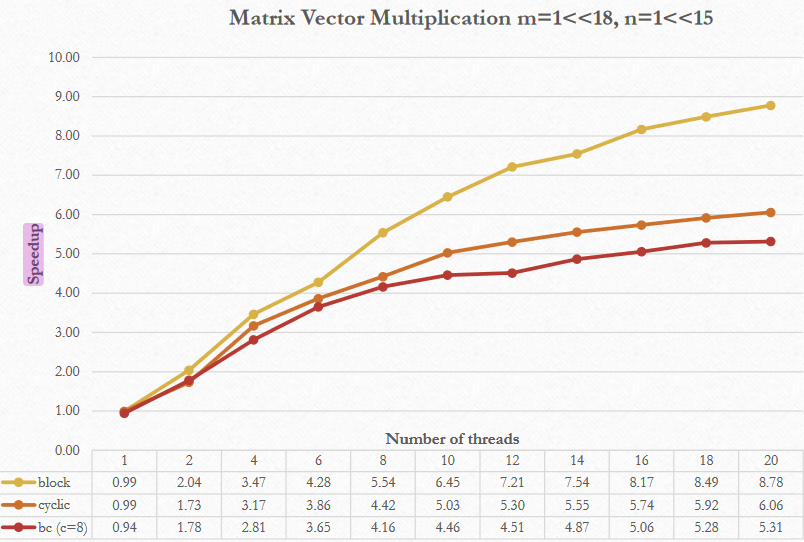
\includegraphics{images/08/speedup}
   \caption{Speedup comparison}
   \label{fig:08/speedup}
\end{figure}

\end{paracol}

\begin{figure}[htbp]
   \centering
   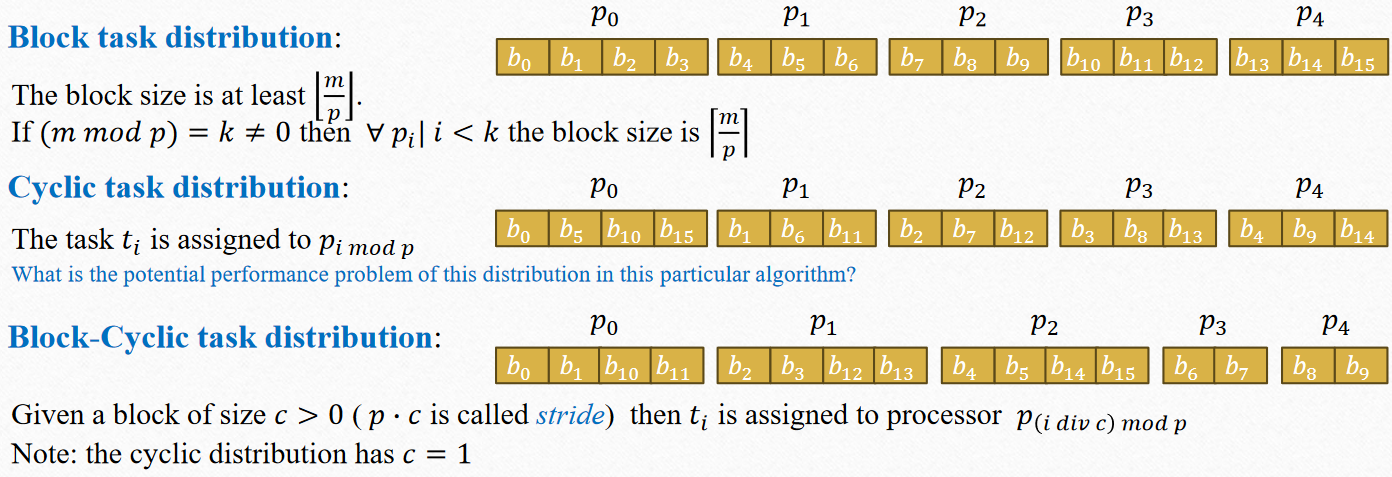
\includegraphics{images/08/static}
   \caption{Static assignment strategies}
   \label{fig:08/static}
\end{figure}

\subsection{Dynamic assignment}

It may not be possible to know in advance how much work each task will have to do. 
The size of the problem may be unkown, or the workload may be unbalanced, meaning that some tasks may result in more work than others.
Even in the case of multiplying matrices, the workload may be strongly unbalanced if the matrices are sparse.

For such cases, dynamic assignment is more appropriate. The master thread assigns work to the worker threads as they become available. This is done by using a \textbf{work queue}.

\framedt{All-pairs distance Matrix}{
   \begin{itemize}
      \item We have a $m\times n$ matrix $D_{ij}$ where $i$ denotes one of the $m$ vectors and $j$ enumerates the $n$ elements of the vector.
      \item We want to compute the distance (or \textit{similarity}) $d(\cdot,\cdot)$ between all pairs of vectors.
      \begin{itemize}
         \item $\Delta_{ij} = d(x^{(i)}, x^{(i')}) \quad = \sqrt{\sum_{k=1}^{n} (D_{ik} - D_{jk})^2}$
         \item The distance/similarity measure $d(\cdot,\cdot)$ might be a traditional metric such as Euclidean distance or any symmetric binary function that assign a notion of similarity to pair of instances
      \end{itemize}
      \item We have to comput $m^2$ distances, so $\mathcal{O} (m^2n)$ operations
      \item However note that $\Delta_{ij} = \Delta_{ji}$, i.e. it is a symmetric matrix, so we can compute only the lower triangular part
   \end{itemize}
}

\begin{paracol}{2}
   We statically assign each row to a thread, using a block cycling distribution.
   This is not ideal, as some rows may take longer to compute than others, resulting in unbalanced workloads.

   In Fig. \ref{fig:08/delta_static} we can see the distribution of the workload. Each row is assigned to a thread, and the workload is distributed in blocks size $c = 2$.
   As $c$ increases, the number of blocks decreases, and the workload becomes more unbalanced.

   \switchcolumn

   \begin{figure}[htbp]
      \centering
      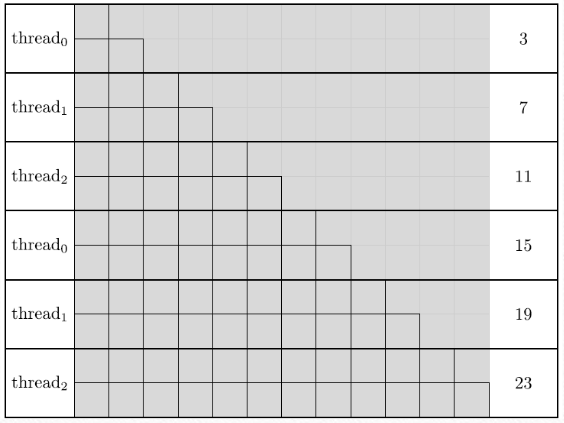
\includegraphics{images/08/delta_static.png}
      \caption{Block cyclic distribution}
      \label{fig:08/delta_static}
   \end{figure}
\end{paracol}

\begin{paracol}{2}
   Consider the snippet on the right. Each thread tries to hold a lock on the mutex, and then updates the global variable \lstinline|lower| with the next row to compute. The global variable \lstinline|global_lower| is updated by the master thread.

   This is a simple example of dynamic assignment, directly performed by thread and automatically balancing the workload. This however comes at the cost of the mutex overhead, which is not negligible.

   In general, if the \ul{workload is not-so-unbalanced, static assignment is preferable}.
   
   \switchcolumn

   \begin{lstlisting}[caption={spm3/all-pairs.cpp}]
// while there are still rows to compute
while (lower < rows) {
   
   // update lower row with global lower row
   {
      std::lock_guard<std::mutex> lock_guard(mutex);
      lower  = global_lower;
      global_lower += chunk_size;
      }
   \end{lstlisting}
         
\end{paracol}


\subsubsection{Producer-Consumer model}
Here we have a shared data structure, typically a queue, that is accessed by multiple threads. The producer thread(s) insert data into the queue, while the consumer thread(s) remove data from the queue. The producer and consumer threads are synchronized by a mutex and a condition variable.

\paragraph{Stop token}

The \lstinline|std::stop_token| is a mechanism to signal the threads to stop. The producer thread will keep adding data to the queue until the stop token is requested. The consumer thread will keep consuming data from the queue until the stop token is requested.

It is not always the way-to-go solution to stop threads, it is one of the available options.
Another option is to use a global \lstinline|std::atomic<bool>| flag, which is more efficient but less flexible.
Or, as I did in my Operative Systems project, to insert a \textit{special value} in the queue to signal the end of the data. 
   
   \begin{lstlisting}[caption={spm3/prod-cons.cpp}]
std::stop_token stoken = stopSrc.get_token();
// ...
auto producer = [&](const std::stop_token &stoken, int id) {	   
	uint64_t i=0;
	while (!stoken.stop_requested()) {
		{
			std::lock_guard<std::mutex> lock(mtx);
			dataq.push_back(i++);
		}
		cv.notify_one();
      //...

auto consumer = [&](const std::stop_token &stoken, int id) {
	std::unique_lock<std::mutex> lock(mtx, std::defer_lock);
	for(;;) {
		lock.lock();
		if (cv.wait(lock, stoken, [&dataq] { return !dataq.empty(); })) {
			auto data = dataq.front();
			(void)data;
			dataq.pop_front();
			//std::printf("Consumer%d, data=%lu\n", id, data);
		}
		else {
			if (stoken.stop_requested()) {
				lock.unlock();
				break;
			}
		}
		lock.unlock();
      // ...
\end{lstlisting}

\newpage
\subsubsection{Multiple-Reader Single-Writer}

A reader may access the data concurrently with
other readers, while a writer needs exclusive access to the shared data.
This is a common pattern with a simple  ---not trivial--- solution.

\begin{paracol}{2}
   
   \colfill
   Using a normal \lstinline|std::mutex| to protect the accesses to the critical section \textbf{does prevent} the concurrent access of multiple readers, so it is not a viable solution.
   The Standard library offers a solution with \lstinline|std::shared_mutex|, which allows multiple readers to access the data concurrently, while a writer needs exclusive access to the shared data.
   \colfill
   
   \switchcolumn   
   
   \begin{lstlisting}[caption={spm3/reader-writer.cpp}]
auto reader = [&](int count, int id) {
   for(int i=0;i<count; ++i) {
      std::shared_lock<std::shared_mutex> lock(smutex);
      std::printf("Reader%d has read %d\n", id, shared_counter);
   }
};
auto writer = [&](int count, int id) {
   for(int i=0;i<count; ++i) {
      std::unique_lock<std::shared_mutex> lock(smutex);
      ++shared_counter;
      std::printf("Writer%d has written %d\n", id, shared_counter);
   }
};  
\end{lstlisting}
               
\end{paracol}

\subsubsection{Thread Pool}
Instead of creating threads on the fly, we can create a pool of threads that are ready to execute tasks. This is useful when the overhead of creating threads is high, and we want to reuse threads for multiple tasks.

There is no out-of-the-box solution of a Thread Pool (TP) in the Standard Library. There are many libraries that provide thread pools, such as \textit{Boost} or \textit{Intel TBB}, but we can also manage them by ourselves.

The synchronization is handled through mutex and condition variables, in a Producer-Consumer fashion.
In the \ul{implementation provided (\texttt{threadPool.hpp}) the task queue is \textbf{unbounded}!}
If the producers are much faster than the Workers, the tasks queue becomes huge, and the memory blows up \frownie.\\
To avoid this we can either increase the number of Worker threads (if we have enough cores), or we can implement a \textbf{bounded queue}.

\section{Lock-Free Programming}
With locks and mutexes, we can ensure that only one thread accesses a critical section at a time. However, this comes at a cost: the overhead of acquiring and releasing the lock, and the possibility of deadlocks.\\
Aside from the operational overhead, the lock approach sometimes forces to spend a lot of time waiting for the lock to be released, even when the critical section is accessed for a very short time.

\subsection{Atomic Counting}
C++11 introduces atomic data types that can be safely manipulated in a concurrent context without acquiring time-consuming locks.
The atomic data types are implemented using hardware instructions that guarantee atomicity.

\begin{lstlisting}[caption={spmcode4/atomic\_counting.cpp}]
   auto lock_count =
        [&] (volatile uint64_t* counter, const auto& id) {
        for (uint64_t i = id; i < num_iters; i += num_threads) {
            std::lock_guard<std::mutex> lock_guard(mutex);
            (*counter)++;
        }
    };
   auto atomic_count =
   [&] (volatile std::atomic<uint64_t>* counter, const auto& id) {
   for (uint64_t i = id; i < num_iters; i += num_threads)
       (*counter)++;
   };

   // > elapsed time (mutex_multithreaded): 5.98232s
   // > elapsed time (atomic_multithreaded): 1.02452s
\end{lstlisting}

\lstinline|std::atomic<T>| is a template class that provides atomic operations on the type \lstinline|T|. The operations are implemented using hardware instructions that guarantee atomicity.\\
\begin{itemize}
	\item \lstinline|std::atomic| is neither copyable nor movable
	\item \lstinline|T| must be copyable and movable
	\item \lstinline|T| cannot have a user-defined copy constructor
	\item Operations (i.e., the methods of the \lstinline|std::atomic| class)
	      \begin{itemize}
		      \item \lstinline|load|/\lstinline|store|: to get and set the content of a \lstinline|std::atomic|
		      \item \lstinline|exchange|: stores a new value and returns the old value
		            of the variable
		      \item \lstinline|compare| and exchange: it does an atomic exchange
		            only if the value is equal to the provided expected value
		      \item \lstinline|wait|/\lstinline|notify| (from C++20) behavior similar to condition
		            variables
	      \end{itemize}
\end{itemize}

\begin{paracol}{2}
   \begin{lstlisting}
   // While there are still rows to compute
   while (lower < rows) {
      // Update lower row with global lower row
      {
         std::lock_guard<std::mutex> lock_guard(mutex);
         lower = global_lower;
         global_lower += chunk_size;
      }
   }
   \end{lstlisting}
   
   \switchcolumn
   
   \begin{lstlisting}
   // While there are still rows to compute
   while (lower < rows) {
      // Update lower row with global lower row
      lower = std::atomic_fetch_add(&global_lower, chunk_size);
   }
   \end{lstlisting}

\end{paracol}

\begin{paracol}{2}
   
   Not all \lstinline|std::atomic| operations are supported on all types. For example, \lstinline|std::atomic<bool>| does not support \lstinline|fetch_add|, but only \lstinline|fetch_or|, \lstinline|fetch_and|, \lstinline|fetch_xor|, and \lstinline|exchange|.
   
   \switchcolumn

   \begin{figure}[htbp]
      \centering
      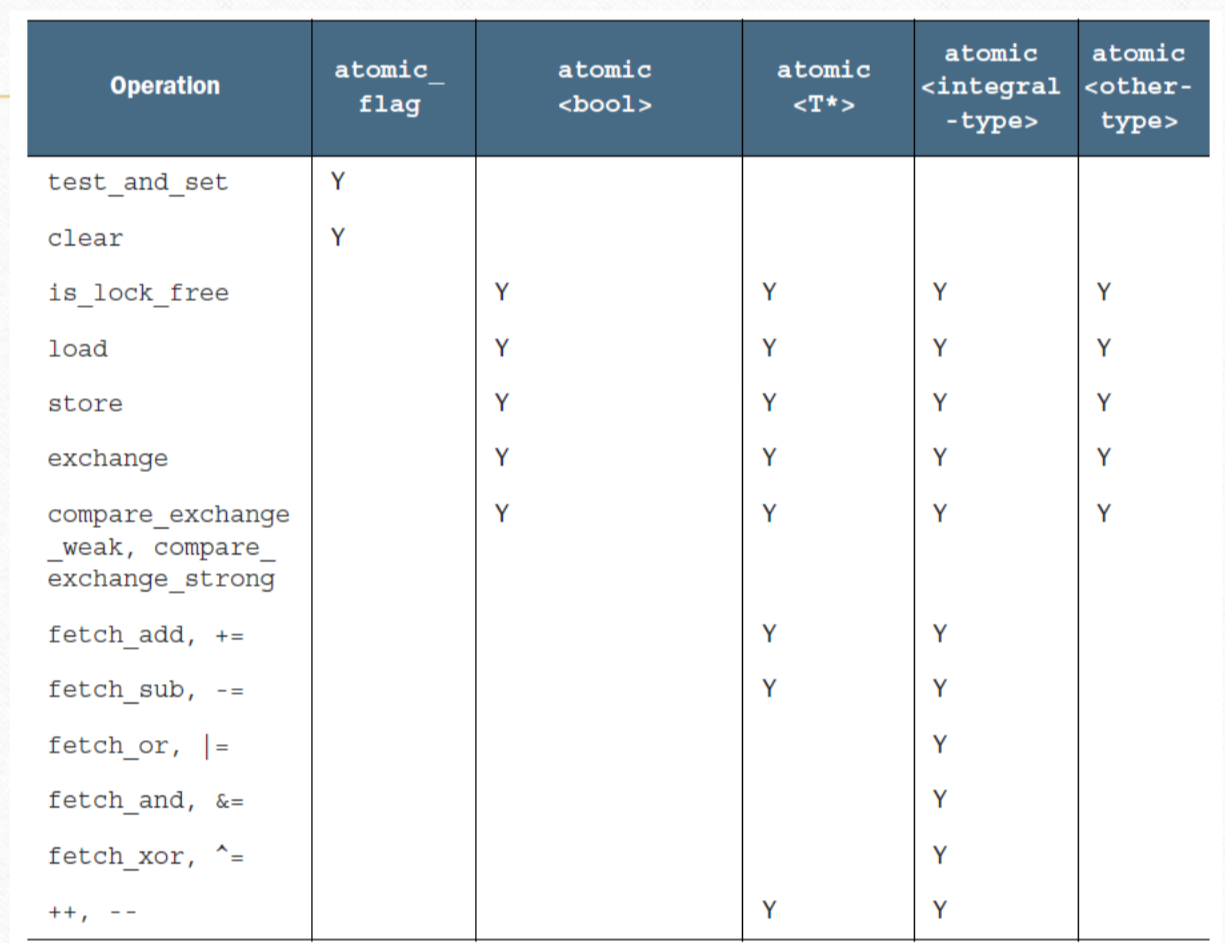
\includegraphics{images/08/atomic_ops.png}
      \caption{Atomic operations supported by std::atomic}
      \label{fig:08/atomic_ops}
   \end{figure}
\end{paracol}

\subsubsection{CAS - Compare and Swap}
Every C++ atomic data type features a CAS (Compare And Swap) operation for implementing arbitrary atomic assignments.
There are two methods for CAS which \ul{should \textit{always} be both performed in loops}:
\begin{itemize}
   \item \lstinline|compare_exchange_weak(T& expected, T desired)|: It may fail spuriously, but it is more efficient
   \note{i.e. may return false even if the comparison yields true}
   \item \lstinline|compare_exchange_strong(T& expected, T desired)|: It unlikely fails spuriously, but it is less efficient
\end{itemize}

\begin{enumerate}
	\item Compare the value expected with the value stored in the atomic
	\item If yes, then it sets the atomic to the value desired, otherwise writes the actual value stored in atomic into expected
	\item Return \textit{true} if the swap operation in step 2 was successful, \textit{false} otherwise
\end{enumerate}

\begin{paracol}{2}
\begin{lstlisting}[caption={Finding the max in an array}]
   auto false_max = [&] (volatile std::atomic<uint64_t> &counter,
                          const auto& id) -> void {
        for (uint64_t i = id; i < num_iters; i += num_threads) {
            if(i > counter) counter = i;
		}
    };
    auto correct_max = [&] (volatile std::atomic<uint64_t> &counter,
                            const auto& id) -> void {
        for (uint64_t i = id; i < num_iters; i += num_threads) {
            auto previous = counter.load();
            while (previous < i &&
                !counter.compare_exchange_weak(previous, i)) {}
        }
    };
\end{lstlisting}

\switchcolumn

The problem with the first uncorrect max implementation is that it is not thread-safe: the \lstinline|load| (reading \lstinline|i<counter|) and \lstinline|store| (writing \lstinline|counter=i|) operations are atomic per se, but anything may happen in between them.\\
For this reason we need to use the CAS operation, which is a \textit{read-modify-write} operation.
\end{paracol}

\section{Memory Consistency Concepts}
The intuition says that a memory read should return \textit{the latest value written} in a memory location.
What does ``\textit{the latest value written}'' mean in a CMP system when executing multiple threads?\\
It depends on the ordering of memory operations, precisely the order in which memory operations
performed by one thread become visible to other threads.
\note{Modern CMPs reorder memory operations in different/strange ways for performance reasons}
Memory consistency defines the allowed behavior of reads and writes (i.e., loads and stores) to
different addresses in a parallel system.

We should care about memory ordering mostly because it helps to program lock-free concurrent code.

Memory consistency deals with when writes to a variable X propagate to other processors relatively to reads and writes to other addresses.

\begin{lstlisting}
   // initially, A = B = flag = 0
   // Thread1 
   Store A = 1;
   Store B = 1;
   Store flag = 1;
   
   // Thread2
   while (Load flag==0); // spin
   Load A;
   Load B;
   print A and B;
\end{lstlisting}

If there are caches in the system, from the viewpoint of the cache coherence protocol, the printing of \lstinline|A=B=0| can be perfectly fine, due to the ordering of instructions, even if we expect that Thread2 should print \lstinline|A=B=1|.

\textbf{Memory consistency} defines correct program behavior and is part of the specification of architectures.
\textbf{Cache coherence} is a different concept, it deals with the objective of ensuring that the memory
system in a parallel computer behaves as if the caches were not present; coherence is \textit{not} directly visible at the software level, but only as a side effect, e.g. false sharing, superlinear speedup\dots

\subsection{Memory Ordering}
The \textbf{program order} defines a sequence of reads and writes.\\
There are four types of memory operation ordering that can be guaranteed (or not) by the platform:
\begin{enumerate}
   \item $W_X \rightarrow R_Y$: write to $X$ must commit before the subsequent read of $Y$
   \note{i.e., when a write comes before a read in program order, the write must commit (i.e, its result must be visible) by the time the read occurs}
	\item $R_X \rightarrow R_Y$: read from $X$ must commit before the subsequent read from $Y$
	\item $R_X \rightarrow W_Y$: read from $X$ must commit before the subsequent write to $Y$
	\item $W_X \rightarrow W_Y$: write to $X$ must commit before the subsequent write to $Y$
\end{enumerate}

\subsubsection{Sequential Consistency - SC}
The most intuitive memory model is \textbf{Sequential Consistency} (SC). It is the most restrictive memory model; it was introduced by Leslie Lamport in 1979.
\begin{definition}
   [Sequential Consistency]
   A multiprocessor is sequentially consistent if the result of any execution is the same as if the operations of all the processors were executed in some sequential order, and the operations of each individual processor appear in this sequence in the order specified by its program.
\end{definition}

Alternatively, \textit{There exists a \textbf{total} order of all loads and stores across all threads such that the value returned by each load is equal to the value of the most recent store to that location}

SC maintains all four memory operation orderings.

\subsubsection{Relaxed Memory Consistency}
The disadvantage to SC is that the firmware may not apply optimizations in the code, which can lead to a significant performance loss. In all modern systems, some reordering and optimizations are enforced.

Relaxed memory consistency models allow the compiler and hardware to violate certain memory ordering rules to improve performance.\\
Ideally, it aims to gain performance by hidinh memory latency, i.e. overlapping memory access operations with other operations when they are independent.

Modern architectures exploit \textit{Write Buffers}, which allow to write to a buffer instead of directly to memory, and \textit{Read Buffers}, which allow to read from a buffer instead of directly from memory.\\
The $W_X \rightarrow R_Y$ ordering is relaxed to hide write latency, hence the processor $k$ may move its own reads ahead of its own writes.
This is fine from the viewpoint of a single-thread control flow.

\begin{paracol}{2}
   \colfill
   \textit{Total Store Order} (TSO) and \textit{Processor Consistency} (PC) relax $W_X \rightarrow R_Y$ in different ways.
   \nl
   
   Partial Store Ordering (PSO) relaxes also $W_X \rightarrow W_Y$.
   The processor might reorder write operations in the Write Buffer: one write might be a cache miss, while the other might be a cache hit whose management costs less.
   \note{This is a valid optimization if a program consists of a single instruction stream}
   \colfill
   
   \switchcolumn

   \begin{lstlisting}
      Thread1
      on P0
      A = 1;
      flag=1;
      
      Thread2
      on P1
      while (flag==0) ; //spin
      print A;
   \end{lstlisting}

   Under PSO, P1 may observe the flag change before the write to A is visible, hence printing 0.
   This behavior would not be allowed by TSO and SC.
\end{paracol}

Even more aggressive reordering may allow to overlap multiple reads and writes, Execute reads as early as possible and writes as late as possible to hide memory latency.
An example is the \textit{Weak Ordering} (WO) model, which \ul{relaxes all orderings}.
\texttt{ARM} and \texttt{POWER} architectures are based on a relaxed memory model.

\subsubsection{Solving this nightmare}
Every architecture provides synchronization primitives to make memory ordering stricter.
\textbf{Memory barrier} instructions (also ``fences'') prevent reordering, but they are expensive:
\begin{itemize}
   \item All memory operations must be completed before any memory operation after the barrier can begin
   \item There are different flowers of fences: load fence (RMB), store fence (WMB), mem fence (MB)
\end{itemize}
Besides, there are also the synchronization primitives discussed before which enable ordering on a specific memory address, such as \lstinline|test_and_set|, \lstinline|compare_and_swap|, and all \lstinline|read-modify-write| (RMW) operations.

However, recall also that \ul{if a program is \textit{Data-Race-Free} (DRF), then its behavior is sequentially consistent}, because the reordering won't affect program correctness.
\ul{Properly syncronized programs} via mutexes, barriers, atomics, etc. \ul{are \textbf{DRF}}.

\coolquote{SC does not guarantee DRF!}{prof. Torquati}


\subsubsection{Programming Languages}
We talked about the underlying architecture as the culprit of reordering, but the programming language can also play a role in this.
\ul{The \textbf{compiler} may reorder instructions for performance reasons independengly from the low-
level architectures}.

It is generally accepted that a compiler can reorder ordinary reads from and writes to memory almost arbitrarily, provided \ul{the reordering cannot change the observed single-threaded execution of the code}.\nl

{\ul{C++ provides six memory orderings options for atomic types}, with the default being the stricter \lstinline|std::memory_order_seq_cst|, i.e. sequential consistency.\ns
\begin{enumerate}
	\item \textbf{Sequential consistency}, loads/stores atomic operations happen in the order specified by the program
	\item \textbf{Acquire}, only valid for atomic load operations. It prevents all loads/stores in the current thread from being moved to a position before the current atomic load operation.
	\item \textbf{Release}, only valid for atomic store operations. It prevents all loads/stores in the current thread from being moved to a position after the current atomic store operation.
	\item \textbf{Relaxed}, no restrictions in memory reordering of surrounding load/store operations. Only the atomicity of the actual operation is guaranteed.
	\item \textbf{Acquire-Release}, only valid for atomic exchange and compare-exchange operations (i.e. RMW operations). It is a combination of the Acquire and Release modes, simultaneosly loads the current value in Acquire mode and stores a new value in the atomic variable in Release mode.
\end{enumerate}}

\begin{itemize}
	\item \textbf{Store} operations can have \lstinline|std::memory_order_relaxed|, \lstinline|std::memory_order_release|, or
	      \lstinline|std::memory_order_seq_cst| ordering values
	\item \textbf{Load} operations can have \lstinline|std::memory_order_relaxed|, (\lstinline|std::memory_order_consume| **),
	      \lstinline|std::memory_order_acquire|, or \lstinline|std::memory_order_seq_cst| ordering values
	\item \textbf{RMW} operations can have \lstinline|std::memory_order_relaxed|, (\lstinline|std::memory_order_consume| **),
	      \lstinline|std::memory_order_acquire|, \lstinline|std::memory_order_release|, \lstinline|std::memory_order_acq_rel| or
	      \lstinline|std::memory_order_seq_cst| ordering values
   \item[**] \lstinline|std::memory_order_consume| is somewhat deprecated and not recommended for use since C++17
\end{itemize}

The SC semantics requires a single total ordering over all atomic operations with ordering \lstinline|std::memory_order_seq_cst|. It is the most expensive memory ordering, it requires global synchronization between all threads (enforced by the C++ compiler).

